\documentclass{article}

% Kodranje in podpora slovenščini
\usepackage[T1]{fontenc}        % kodiranje znakov v .pdf
\usepackage[utf8]{inputenc}     % kodiranje znakov v .tex
\usepackage[slovene]{babel}     % nastavimo slovenščino

\usepackage{graphicx} % za vstavljanje slik

\usepackage{booktabs} % za lepše tabele
\usepackage{multirow} % za vnose v tabeli čez več vrstic

\usepackage{siunitx}  % za poravnavo na decimalni vejici v tabeli
\sisetup{output-decimal-marker={,},group-separator={.}}

\usepackage{listings} % za prikaz programske kode

\usepackage{pgfplots} % za risanje grafa funkcije

\title{Slike in tabele}
\author{Andrej Bauer}

\begin{document}

\maketitle

\begin{abstract}
  V članku predstavimo, kako v {\LaTeX}u delamo tabele in kako vstavljamo slike.
\end{abstract}

\section{Okolji \texttt{table} in \texttt{tabular}}
\label{sec:okolje-texttttabular}

V tabeli~\ref{tab:volitve-vanilla} vidimo rezultate volitev, uporabili so navaden {\LaTeX}.
V tabeli~\ref{tab:volitve-booktabs} vidimo rezultate volitev, uporabili smo paket \texttt{booktabs}.
V tabeli~\ref{tab:volitve-align} vidimo rezultate volitev s poravnanimi decimalnimi pikami in vejicami.

% h = here (tukaj)
% t = top (na vrhu strani)
% p = page (na svoji strani)
\begin{table}[htp]
  \centering
  \begin{tabular}{|l|r|r|}
  \hline
  \textbf{Kandidat/Kandidatka}        & \textbf{Odstotek} & \textbf{Število glasov} \\ \hline
  Borut Pahor                & 47,07\%  & 348.938 \\ \hline
  Marjan Šarec               & 24,96\%  & 185.042 \\ \hline
  Romana Tomc                & 13,74\%  & 101.845 \\ \hline
  Ljudmila Novak             & 7,16\%   & 53.049 \\ \hline
  Andrej Šiško               & 2,22\%   & 16.463 \\ \hline
  Boris Popovič              & 1,79\%   & 13.277 \\ \hline
  dr.\ Maja Makovec Brenčič  & 1,72\%   & 12.734 \\ \hline
  Suzana Lara Krause         & 0,77\%   & 5.718 \\ \hline
  Angela (Angelca) Likovič   & 0,58\%   & 4.273 \\ \hline
  \end{tabular}
  \caption{Rezultati predsedniških volitev, kot bi jih prikazali z grdo razpredelnico, ki ima preveč črt.}
  \label{tab:volitve-vanilla}
\end{table}

\begin{table}[htb]
  \centering
  \begin{tabular}{lrr}
  \toprule
  \textbf{Kandidat/Kandidatka}        & \textbf{Odstotek} & \textbf{Število glasov} \\ \midrule
  Borut Pahor                & 47,07\%  & 348.938 \\
  Marjan Šarec               & 24,96\%  & 185.042 \\
  Romana Tomc                & 13,74\%  & 101.845 \\
  Ljudmila Novak             & 7,16\%   & 53.049 \\
  Andrej Šiško               & 2,22\%   & 16.463 \\
  Boris Popovič              & 1,79\%   & 13.277 \\
  dr.\ Maja Makovec Brenčič  & 1,72\%   & 12.734 \\
  Suzana Lara Krause         & 0,77\%   & 5.718 \\
  Angela (Angelca) Likovič   & 0,58\%   & 4.273 \\
  \bottomrule
  \end{tabular}
  \caption{Rezultati predsedniških volitev s paketom \texttt{booktabs}}
  \label{tab:volitve-booktabs}
\end{table}

% V tej tabeli smo števila zapisali 
\begin{table}[htb]
  \centering
  \begin{tabular}{lSS[group-minimum-digits=3]}
  \toprule
  \textbf{Kandidat/Kandidatka}        & \textbf{Odstotek} & \textbf{Število glasov} \\ \midrule
  Borut Pahor                & 47.07\%  & 348938 \\
  Marjan Šarec               & 24.96\%  & 185042 \\
  Romana Tomc                & 13.74\%  & 101845 \\
  Ljudmila Novak             & 7.16\%   & 53049 \\
  Andrej Šiško               & 2.22\%   & 16463 \\
  Boris Popovič              & 1.79\%   & 13277 \\
  dr.\ Maja Makovec Brenčič  & 1.72\%   & 12734 \\
  Suzana Lara Krause         & 0.77\%   & 5718 \\
  Angela (Angelca) Likovič   & 0.58\%   & 4273 \\
  \bottomrule
  \end{tabular}
  \caption{Rezultati predsedniških volitev, s poravnanimi decimalnimi vejicami in pikami}
  \label{tab:volitve-align}
\end{table}

\section{Vnosi čez več vrstic ali stoplcev}
\label{sec:vnosi-ez-ve}

Tu je primer tabele, v kateri smo naredili vnose, ki se raztezajo čez več vrstic in stolpcev.

\begin{center}
\begin{tabular}{lll}
  \toprule
  \multicolumn{3}{c}{Živali} \\ \midrule
  \multirow{3}{*}{Domače} & krava & svinja \\
                          & pes & mačka \\
                          & konj & osel \\
  Divje                   & medved & volk \\ \bottomrule
\end{tabular}
\end{center}

\section{Slike}
\label{sec:slike}

Seveda lahko vstavimo tudi sliko, glej sliki~\ref{fig:muca} in~\ref{fig:kuza}.

\begin{figure}
  \centering
  \includegraphics[width=0.5\textwidth]{muca.jpg}
  \caption{Prvi zadetek na Google za ``the cutest kitten in the world.''}
  \label{fig:muca}
\end{figure}

\begin{figure}[ht]
  \centering
  \includegraphics[width=0.5\textwidth]{kuza.jpg}
  \caption{Prvi zadetek na Google za ``the cutest puppy in the world.''}
  \label{fig:kuza}
\end{figure}


\section{Programska koda}
\label{sec:programska-koda}


Spodaj je prikazana izvorna koda za hitro urejanje (angl.\ quicksort).
V \ref{line:ret}.\ vrstici piše \lstinline|return less + pivotList + more|.
Treba je tudi povedati, da ta implementacija ni ravno najboljša.

\begin{lstlisting}[language=Python,numbers=left,escapechar=|]
def quickSort(arr):
    less = []
    pivotList = []
    more = []
    if len(arr) <= 1:
        return arr
    else:
        pivot = arr[0]
        for i in arr:
            if i < pivot:
                less.append(i)
            elif i > pivot:
                more.append(i)
            else:
                pivotList.append(i)
        less = quickSort(less)
        more = quickSort(more)
        return less + pivotList + more|\label{line:ret}|
 
a = [4, 65, 2, -31, 0, 99, 83, 782, 1]
a = quickSort(a)
\end{lstlisting}

\section{Rišemo s TiKZ}
\label{sec:riemo-s-tikz}

S paketom TiKZ lahko narišemo skoraj vse.
%
\begin{center}
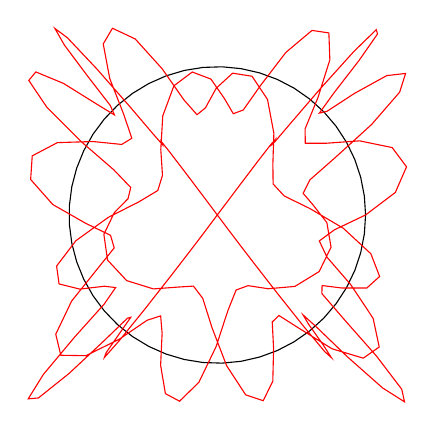
\begin{tikzpicture}
\begin{axis}[
    trig format plots=rad,
    axis equal,
    hide axis
]
\addplot [domain=0:2*pi, samples=50, black] ({cos(x)}, {sin(x)});
\addplot [domain=0:2*pi,samples=200, red]({(1+0.3*sin(24*x))*cos(3*x)},{(1+0.3*sin(24*x))*sin(4*x)});
\end{axis}
\end{tikzpicture}
\end{center}

\end{document}
